% Búsqueda local
La búsqueda local es un método heurístico para mejorar una dada solución factible a un problema. Se basa en, a partir de  una solución inicial $s$, mejorar esa solución iterativamente, tomando la mejor solución de un conjunto de vecinos de $s$. El conjunto de los vecinos se determina mediante algún criterio y se usa una función objetivo para comparar las soluciones en la vecindad de $s$ y discernir cual es la mejor.

La búsqueda local se puede expresar de la siguiente manera:\\\\
\hspace*{1 cm} Sea $s \in S$ una solución inicial\\
\hspace*{1 cm} Mientras exista $s' \in N(s)$ con $f(s') < f(s)$:\\
\hspace*{2 cm} $s \leftarrow s'$

Siendo $N(s)$ la vecindad de $s$ y $f$ la función objetivo que se quiere minimizar. Una versión de la búsqueda local se encarga además de que el vecino que elige minimice la función objetivo entre todas los vecinos.

% Solución inicial
\subsubsection{Solución inicial}

Como solución inicial se utilizó la heurística \texttt{Greedy} desarrollada en el punto anterior, consistente en elegir la mejor de tres corridas del algoritmo de Dijkstra con distintas funciones de peso.

% Definición de la vecindad
\subsubsection{Definición de la vecindad}

En cada iteración definimos la vecindad de $s$, $N(s)$, de la siguiente manera: dado el grafo G, y una solución formada por un camino $c \in G$, definimos sus soluciones vecinas como aquellas resultantes de tomar un subcamino $d_{n_1,n_2} \subseteq c$ entre un par de nodos $n_1,n_2$ cualesquiera, y reemplazarlo por otro camino $d_{n_1,n_2}^*$ en $G$, de tal forma que el camino $c^* = c - d_{n_1,n_2} + d_{n_1,n_2}^*$ resultante cumpla: 

\begin{itemize}
\item $\omega_1(c^*)$ $<=$ $K$
\item $\omega_2(c^*)$ $<$ $\omega_2(c)$
\end{itemize}

De la forma descripta, dada una solución formada por un camino $c$ definimos su vecindad como el conjunto $S^*$ de todos los caminos $c^*$ posibles.

Corremos previamente $n$ veces Dijkstra, desde cada nodo. Guardamos los resultados en una matriz tal que en la posición $[i][j]$ guarda el camino mínimo del nodo $i$ al $j$. Cada camino $d_{n_1,n_2}^*$ es el camino mínimo entre $n_1$ y $n_2$ según $\omega_2$, se obtiene de la matriz. Debe además cumplir $\omega_1(c^*) \leq K$. De todos los $c^*$, se elige el que minimice $\omega_2$. Esto se enmarca en la elección de vecinos utilizando el método \textit{Steepest Descent} consistente en elegir al vecino que minice la función objetivo.

Ahora, para calcular $\omega_2(c^*)$, lo calculamos como

\[
\omega_2(c) - \omega_2(d_{n_1,n_2}) + \omega_2(d_{n_1,n_2}^*)
\]

, valores que ya tenemos calculados.

\subsubsection{Pseudocódigo}

El algoritmo está implementado en la función \texttt{main}:

\begin{algorithm}[H]
\caption{$main$(int tipo\_solucionInicial, Graph g, Nodo n1, Nodo n2)}
\begin{algorithmic}[1]
  \State crearMatrizCaminosMinimos(g)
  \State Solution solucion = \texttt{Greedy(g, n1, n2)}
  
  \If{$\omega_1$(solucion) $\leq$ K}    
    \While{True}    	        
    	\State Solution nuevaSolucion = dameMejorVecino(solucion)
	\If{nuevaSolucion == NULL} 
		\State break	
	\EndIf    
	\State solucion = nuevaSolucion	
    \EndWhile
  \EndIf
\end{algorithmic}
\end{algorithm}

\begin{algorithm}[H]
\caption{$dameMejorVecino$(Solution solucionOriginal)}
\begin{algorithmic}[1]	
          \State Solution mejorSolucion = \&solucionOriginal
	  \State vector<int> nodos = \&nodos(solucionOriginal)
	  \For{i=0; i $<$ size(nodos); i++}
	  	\For{j=i+1; j $<$ size(nodos); j++}
			\State Solution subSolucion = crearSubSolucionEntre(solucionOriginal, nodos[i], nodos[j])
			\State Solution solucion\_ij = dameCaminoResueltoEntre(nodos[i], nodos[j])
			\State Solution nuevaSolucion\_$\omega_2$ = $\omega_2$(solucionOriginal) - $\omega_2$(subSolucion) + $\omega_2$(solucion\_ij)
			\State Solution nuevaSolucion\_$\omega_1$ = $\omega_1$(solucionOriginal) - $\omega_1$(subSolucion) + $\omega_1$(solucion\_ij)			
			\If{nuevaSolucion\_$\omega_2$ $<$ $\omega_2$(mejorSolucion) \&\& nuevaSolucion\_$\omega_1$ $\leq$ K)}
				\State mejorSolucion = crearSolucionReemplazandoCamino(solucionOriginal, solucion\_ij)
			\EndIf
		\EndFor
	\EndFor
	\State return mejorSolucion
\end{algorithmic}
\end{algorithm}

\begin{algorithm}[H]
\caption{$crearSolucionReemplazandoCamino$(Solution orig, Solution sub)}
\begin{algorithmic}[1]	
	 \State Solution res
	 \State res = obtenerCaminoHasta(nodos(sub)[0])
	 \State res += sub
	 \State int subSize = size(nodos(sub))
	 \State res += obtenerCaminoDesde(nodos(sub)[subSize-1])	  
	\State return res
\end{algorithmic}
\end{algorithm}

\fixme{poner la parte de remover caminos en el pseudo del main, y capaz agregar el pseudo de la funcion}
% Complejidad
\subsubsection{Complejidad}

Implementamos el algoritmo en la función $main$. La complejidad del algoritmo resulta la suma de obtener la solución inicial y el ciclo que se usa para mejorarla buscando un mejor vecino en cada iteración. 
Además, en $main$, inicialmente, se llama a una función crearMatrizCaminosMinimos, que abordaremos más adelante.

Para obtener la solución inicial, usamos obtenerSolucionInicial. Esta función devuelve un camino mínimo entre 2 nodos llamando a resolverConDijkstra con alguna función objetivo(Greedy\_A o Greedy\_C). La función resolverConDijkstra primero ejecuta Dijkstra para encontrar todos los caminos mínimos entre n1 y los demás nodos y después hace un recorrido inverso  desde n2 hasta n1 para dar con el camino mínimo entre ellos. Como se comprobó en el apartado anterior, la complejidad de Dijkstra es $O(m log(n))$ y el recorrido inverso es $O(n)$, por lo que en total la complejidad de obtenerSolucionInicial es $O(m log(n))$. Cabe notar que la función objetivo usada en Dijkstra no influye en la complejidad, ya que solo compara los valores de $\omega_1$ y $\omega_2$, por lo que tiene complejidad $O(1)$.

Para mejorar la solución usamos un ciclo y en cada iteración obtenemos el mejor vecino del camino actual usando dameMejorVecino. Ejecutamos el ciclo mientras en la última iteración hayamos encontrado una mejora al camino actual. 
Dado que un vecino consiste en reemplazar la porción del camino actual que une 2 nodos $n_1$ y $n_2$ por el camino mínimo según $\omega_2$ entre ellos, y que cada vez que se hace el reemplazo se disminuye $\omega_2$ del camino actual, se pueden hacer a lo sumo tantos reemplazos como caminos mínimos entre todo par de nodos del grafo existan. 
La cantidad de caminos mínimos entre todo par de nodos de un grafo es $n * (n-1) / 2$, ya que cada nodo tiene un camino mínimo hacia todos los demás y no a sí mismo. Esto es, si hay n nodos, el nodo $n_1$, tiene un camino mínimo hacia los nodos $n_2$, ..., $n_n$, el nodo $n_2$ tiene un camino hacia $n_3$, ..., $n_n$ ya que no se vuelve a contar el camino entre $n_1$ y $n_2$ y así hasta $n_{n-1}$ que tiene un camino hasta $n_n$.
Luego, la cantidad máxima de iteraciones es $n * (n-1) / 2$.

Para analizar la complejidad de cada iteración hay que analizar la complejidad de dameMejorVecino. 
Lo primero que hace la función es obtener el arreglo de nodos de la solución pasada por parámetro, que llamamos solucionOriginal. Cómo el camino de solucionOriginal está representado como una lista de ejes, lo que hace es iterar por todos los ejes y tomar el nodo1 del eje y al final adicionar el nodo2 del último eje. Por ende, tomando $t$ como la cantidad de nodos en el camino, en cada iteración, por cada eje del camino, se toma un nodo y esto se hace $t$-1 veces y luego se añade el nodo final. Como $t$ puede ser a lo sumo $n$, entonces la complejidad de esto resulta $O(n^2)$.
Luego de ejecuta un doble $for$ de $t * (t-1) / 2$ iteraciones, que en cada iteración intenta mejorar el mejor camino encontrado hasta el momento, que llamamos mejorSolucion. Inicialmente mejorSolucion es igual a solucionOriginal. 
Para encontrar una mejor solución en cada iteración hacemos lo siguiente:

\begin{itemize}
\item Creamos el subcamino de solucionOriginal entre los nodos $n_1$ y $n_2$.
\item Obtenemos el camino mínimo entre los nodos $n_1$ y $n_2$.
\item Obtenemos un nuevo camino reemplazando el el subcamino entre los nodos $n_1$ y $n_2$ por el camino mínimo entre ellos.
\end{itemize}

Para crear el subcamino de solucionOriginal entre $n_1$ y $n_2$ usamos crearSubSolucionEntre. Esta función recibe un par de nodos y un camino y devuelve el subcamino que une a los nodos. Para esto tiene que recorrer a lo sumo todos los nodos del camino, o sea $t$, que puede ser a lo sumo $n$.

Para obtener el camino mínimo entre los nodos $n_1$ y $n_2$ usamos una optimización que es que en la función $main$, al comienzo, ejecutamos crearMatrizCaminosMinimos que crea una matriz de caminos mínimos entre todo par de nodos del grafo. Generamos esta matriz ejecutando Dijkstra para todos los nodos usando como función objetivo $\omega_2$. Usamos esta matriz para obtener en $O(1)$ el camino mínimo entre los nodos $n_1$ y $n_2$.
Como crearMatrizCaminosMinimos ejecuta un Dijkstra por cada nodo, su complejidad es $O(n * (m log n))$.

Para obtener el nuevo camino reemplazando el subcamino entre $n_1$ y $n_2$ por el camino mínimo entre ellos, usamos crearSolucionReemplazandoCamino.
Lo que hacemos es generar una nueva solución que es la concatenación de 3 caminos: el camino mínimo entre $n_1$ y $n_2$ y los dos pedazos del camino original sin el subcamino que unía $n_1$ y $n_2$. Para crear el camino, hay que recorrer el solucionOriginal y añadir todos los nodos hasta $n_1$ y luego añadir todos los nodos del camino mínimo y al final añadir todos los nodos desde $n_2$ hasta el final de solucionOriginal. Por ende es como iterar sobre el nuevo camino que a lo sumo puede tener $n$ nodos y por ende la complejidad resulta $O(n)$.

Entonces, resulta ser que encontrar el mejor vecino, consiste en ejecutar el doble $for$ de algo que tiene complejidad $O(n + 1 + n)$, o sea $O(n)$, entonces en total es $O(n^2 * n) = O(n^3)$.

Como habíamos explicado que dameMejorVecino se ejecuta en un ciclo de hasta $n * (n-1) / 2$ iteraciones, o sea $O(n^2)$, y entonces resulta que la complejidad de encontrar el mejor vecino es $O(n^2 * n^3) = O(n^5)$. 

Finalmente la complejidad total resulta ser la suma de las complejidades de crearMatrizCaminosMinimos, 2 veces obtenerSolucionInicial y $n^2$ veces dameMejorVecino. Es decir, $O(n * (m log n) + 2 * (m log n) + n^5) = O(n^5)$.

% Familias malas
\subsubsection{Familias malas}

Si elegimos como solución inicial a la heurística Greedy B en la sección previa, se ha expuesto que puede fallar en el intento de dar una solución factible, aún existiendo una. El Greedy A siempre encuentra una solución factible de existir ésta. 

Veamos que tomando nuestra heurística de búsqueda local como solución inicial, puede quedar arbitrariamente lejos de la solución óptima.

Presentamos la siguiente familia de grafos:

\ponerGrafico{imagenes/maloLocalA.png}{}{0.5}{malo-para-local-a}

Para ir de 1 a 5 hay tres caminos posibles: ($C_1$) $1 \rightarrow 2 \rightarrow 5$; ($C_2$) $1 \rightarrow 3 \rightarrow 5$;
($C_3$) $1 \rightarrow 4 \rightarrow 5$;

\begin{eqnarray}
 \omega_1(C_1) &=& 4	\\ 
 \omega_2(C_1) &=& 2	\\
 \omega_1(C_2) &=& 2	\\
 \omega_2(C_2) &=& 2x   \\
 \omega_1(C_3) &=& 6	\\
 \omega_2(C_3) &=& 1
\end{eqnarray}

Supongamos que K vale 4.
Como decíamos, partimos del camino mínimo entre $u$ y $v$ de acuerdo a $\omega_1$, $C_2$. El algoritmo va a intentar intercambiar $C_2$ por
$C_3$, el camino que minimiza $\omega_2$. Sin embargo, como éste se pasa del límite K, el algoritmo no puede seguir y devuelve $C_2$. Sin
embargo $C_1$ era una solución mejor.

$\frac{\omega_2(C_2)}{\omega_2(C_1)} = x$.

Haciendo crecer el valor de $x$ podemos encontrar grafos en los que nuestro algoritmo devuelve una
solución arbitrariamente lejos de la óptima.

\newpage
\subsubsection{Experimentación}

Pudimos analizar el tiempo de ejecución frente a grafos de un tamaño considerable. A continuación presentamos un gráfico.

\begin{figure}[H]
\begin{center}
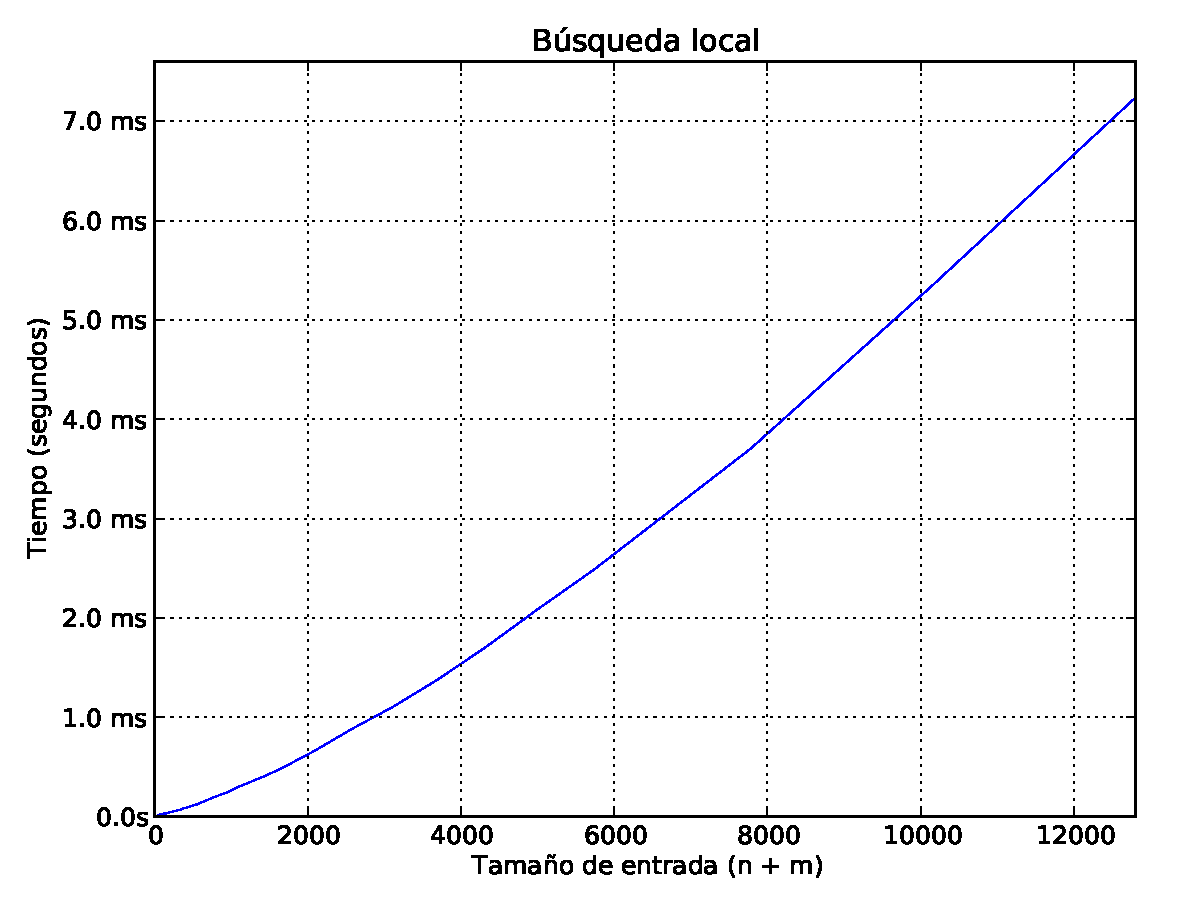
\includegraphics[angle=0, scale=.75]{imagenes/local_search_time.pdf}
\label{grafico local}
\end{center}
\end{figure}


Se puede percibir el carácter no lineal de la complejidad. Sin embargo no se evidencia a luces claras la cota teórica de $n^5$ desarrollada
previamente. Puede ser necesario un tamaño mayor para poder apreciar esa complejidad, o quizás la cota teórica no se alcanza en la práctica.
Probablemente haya un factor que se amortice, habiendo escapado de nuestro escrutinio.

Experimentamos con distintas densidades de grafos. Primero con grafos densos, es decir con una cantidad de aristas del orden de $n^2$. Luego con
grafos de densidad media, con una cantidad de aristas del orden de $\sqrt{n}*n$. Finalmente probamos con grafos ralos, con una cantidad de aristas
del orden de la cantidad de nodos. Para cada grupo de grafos, analizamos diferentes rangos de tamaños de entrada, con el objetivo de demostrar
que el algoritmo mantiene ciertas propiedades, más allá del tamaño.

Se generan cien instancias para cada tamaño de entrada. En los siguientes gráficos se pueden observar comparados el mejor resultado, el peor
resultado, y el resultado promedio para cada tamaño de entrada.

\begin{figure}[H]
\begin{center}
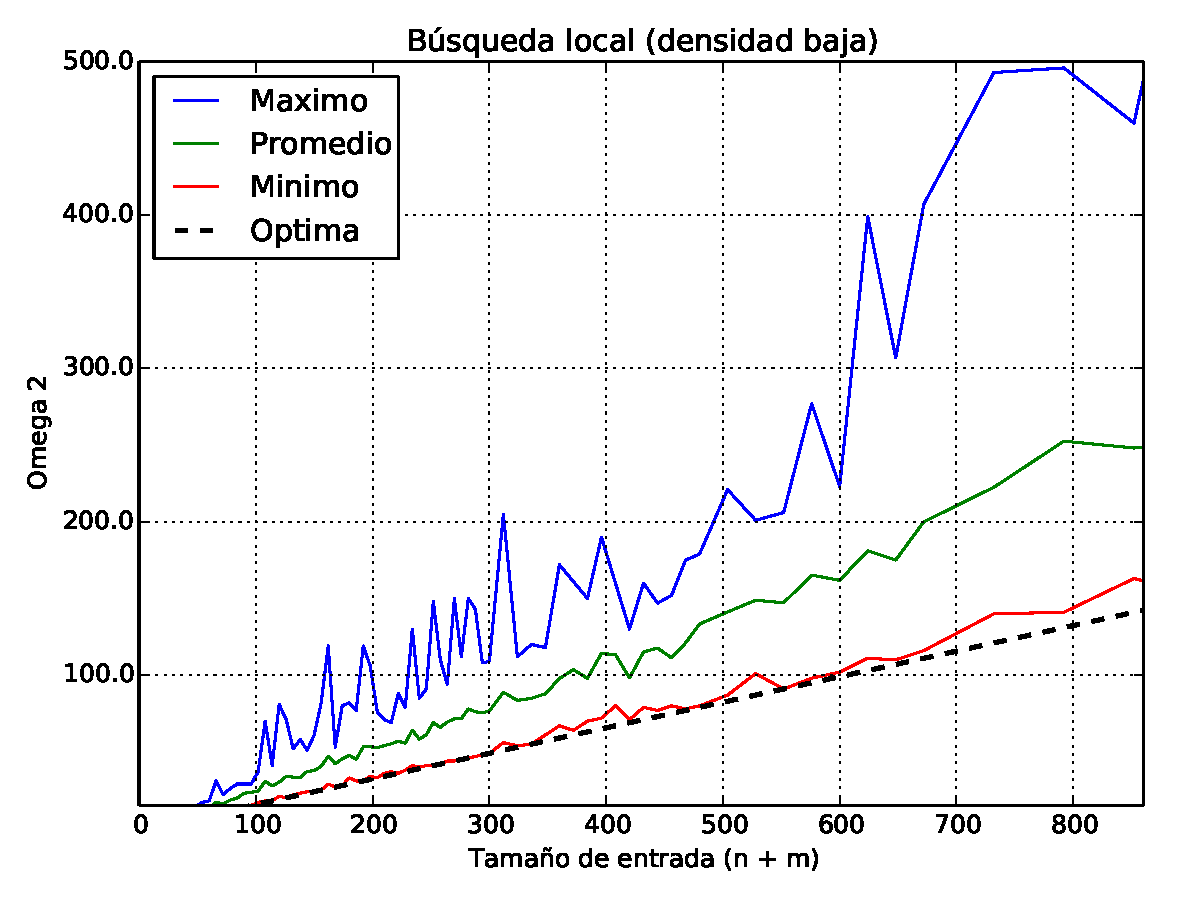
\includegraphics[angle=0, scale=.75]{imagenes/calidad_local_search_2014-06-27_16-02-57.pdf}
\label{grafico local}
\end{center}
\end{figure}

\begin{figure}[H]
\begin{center}
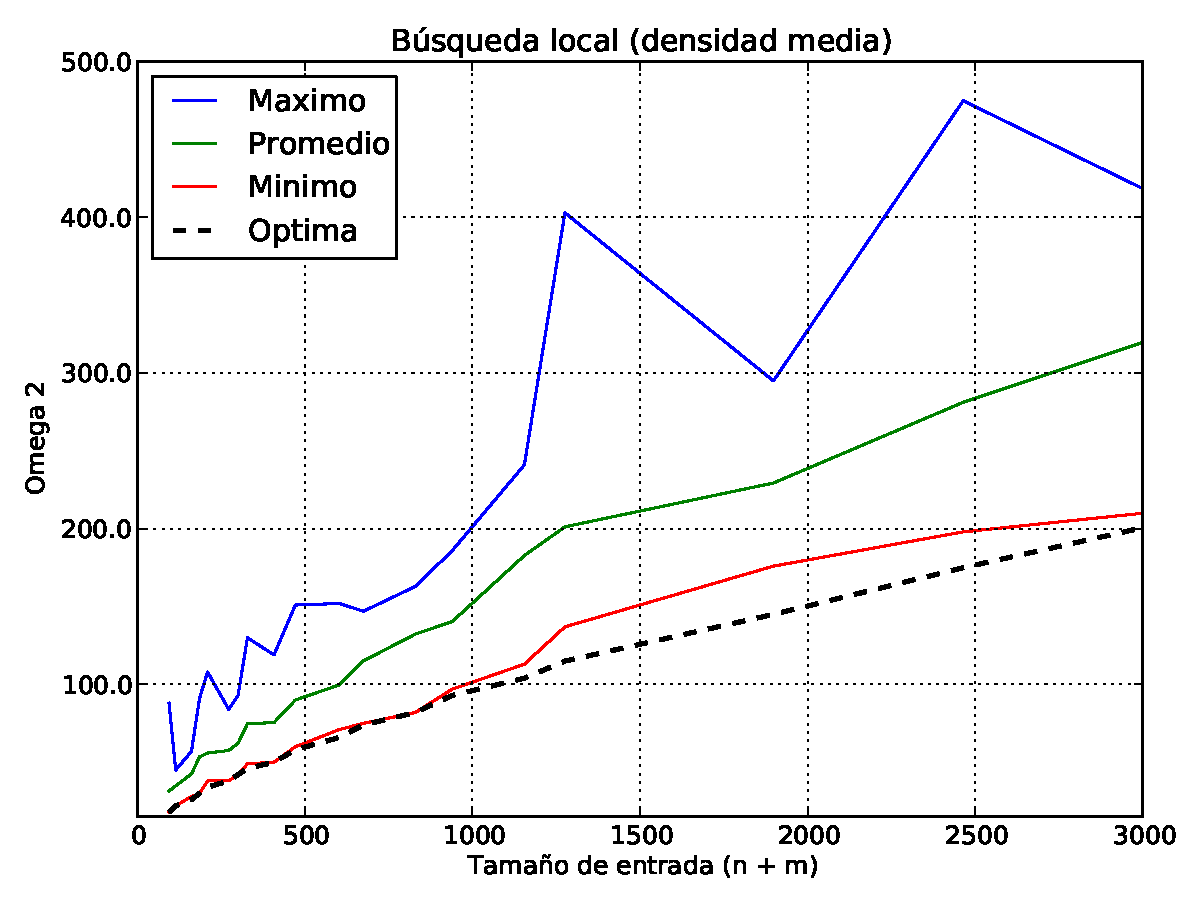
\includegraphics[angle=0, scale=.75]{imagenes/calidad_local_search_2014-06-27_08-58-52.pdf}
\label{grafico local}
\end{center}
\end{figure}

\begin{figure}[H]
\begin{center}
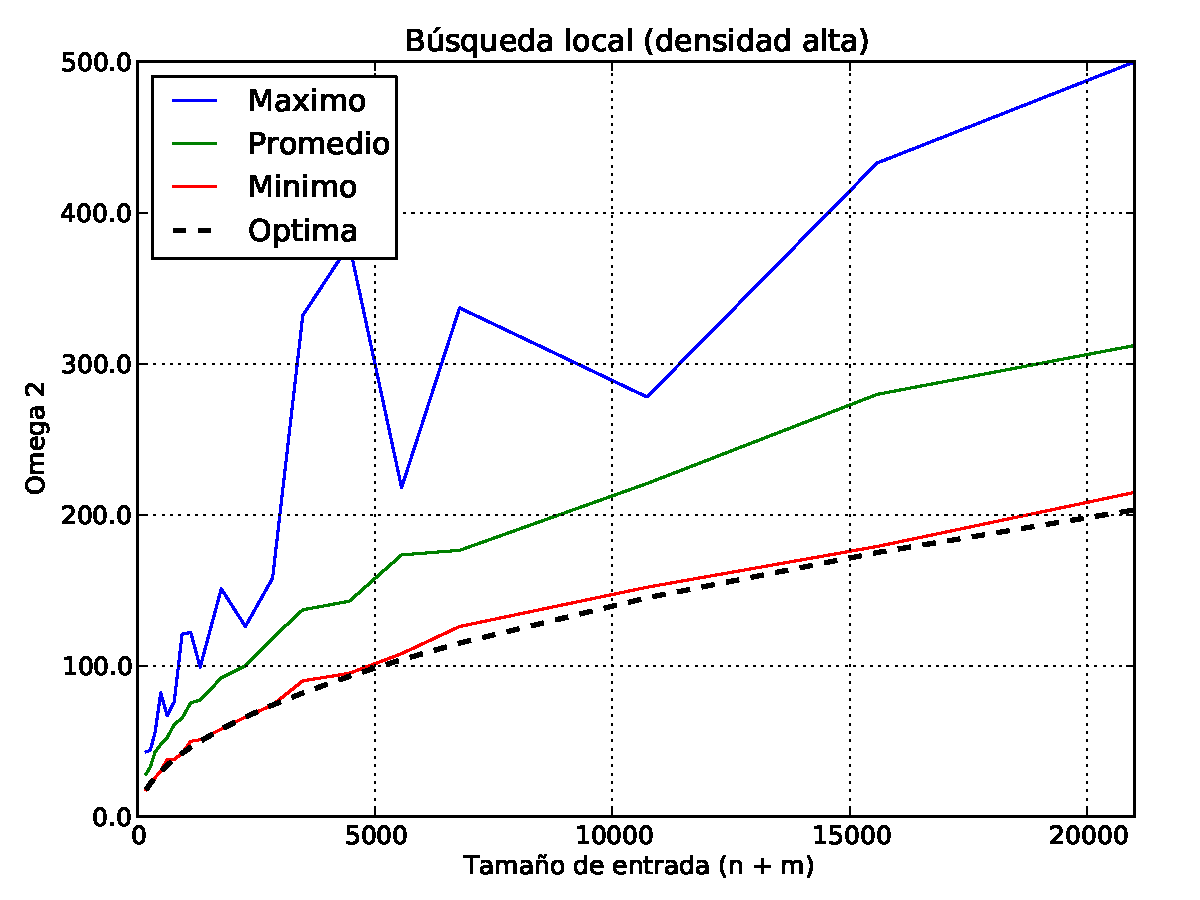
\includegraphics[angle=0, scale=.75]{imagenes/calidad_local_search_2014-06-27_08-54-45.pdf}
\label{grafico local}
\end{center}
\end{figure}

En los tres gráficos se puede notar, a medida que aumenta el tamaño de la entrada, una mayor amplitud de resultados. Ésto tiene cierta intuición. 
Se generan muchas instancias para cada tamaño. A medida que aumenta la cantidad de aristas y vértices, aumenta la variedad entre las instancias
generadas. Por eso se puede ver una gran diferencia de resultado entre instancias del mismo tamaño.
La solución media, no obstante, parece preservar cierta distancia relativa a la solución óptima.
La mejor solución encontrada siempre está muy cerca de la solución óptima. Ésto se evidencia particularmente en el tercer gráfico, lo que
atribuímos a la mayor densidad que le permite al algoritmo tener una vecindad amplia para recorrer.
